\documentclass[main.tex]{subfiles}

\begin{document}
\chapter{Parallelization of DFPT calculations}\label{ch:optimization_ph}

The \texttt{PHonon} package enables calculations of phonon eigenvectors and eigenmodes.
This chapter examines the best ways to run \texttt{PHonon} calculations.

\section{Optimal parallelization parameters for DFPT calculations}

As discussed in sec. \ref{sub:qe_parallelization}, the \texttt{PHonon} package offers the same three parallelization levels as the \texttt{PWscf} package, namely plane wave, k point and linear algebra parallelization.
Furthermore parallelization on q points (so called image parallelization) can be used.

\subsection{k point parallelization}

In a first step, the same k point parallelization benchmark as in sec. \ref{sub:scf_scaling_k_point} is run. This is depicted in fig. \ref{fig:scaling_ph_nk_si}.

\begin{figure}[h!]
    \centering
    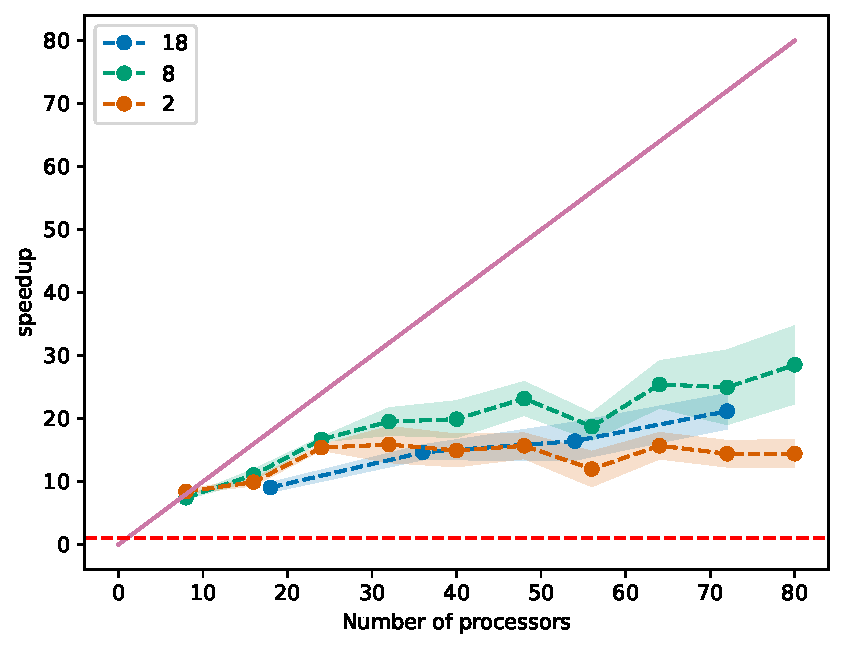
\includegraphics[width=0.75\textwidth]{plots_ph/si_ph_bench_nk_speedup.pdf}
    \caption{Scalability utilizing k-point parallelization for the Si benchmarking system with three sizes of processor pools, \emph{\QE compiled with \gls{oneapi} 2021.4, \texttt{nd 1}}}
    \label{fig:scaling_ph_nk_si}
\end{figure}
Interestingly, the result from the \texttt{PWscf} calculation on silicon from sec. \ref{sub:scf_scaling_k_point} is not reproduced here: the smallest pool size of 2 is not the one parallelizing best, but instead it is pool size 8.
Furthermore, for more than 50 processors, even the biggest pool size 18 shows better scaling than the pool size 2.
This is similar to the results in the \texttt{PWscf} benchmark with k point parallelization on the \TaS benchmarking system in sec. \ref{sub:scf_scaling_k_point}, as the separation between the different pool sizes isn't as clear as in the same benchmark on the silicon benchmarking system.

\todo{some more interpretation possible}

\begin{figure}[htb!]
    \centering
    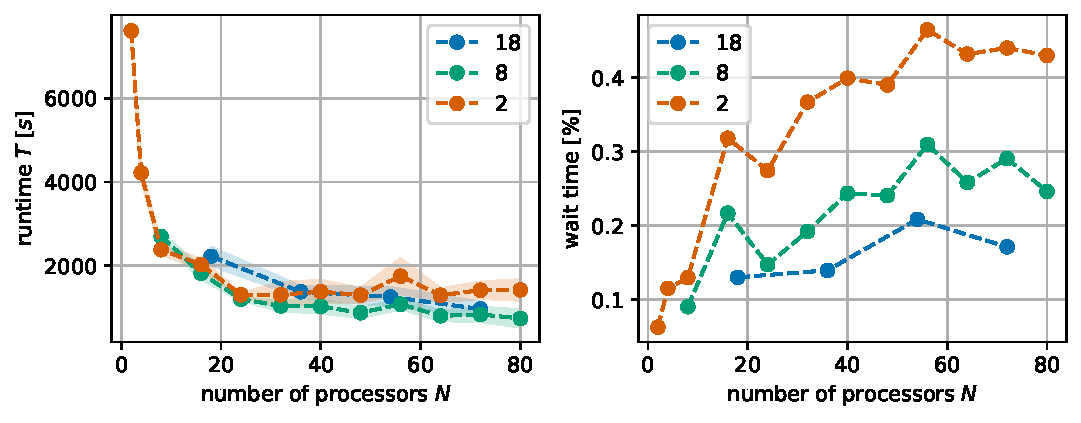
\includegraphics[width=\textwidth]{plots_ph/si_ph_bench_nk_absolute_wait.pdf}
    %\begin{subfigure}[b]{0.49\textwidth}
    %    \centering
    %    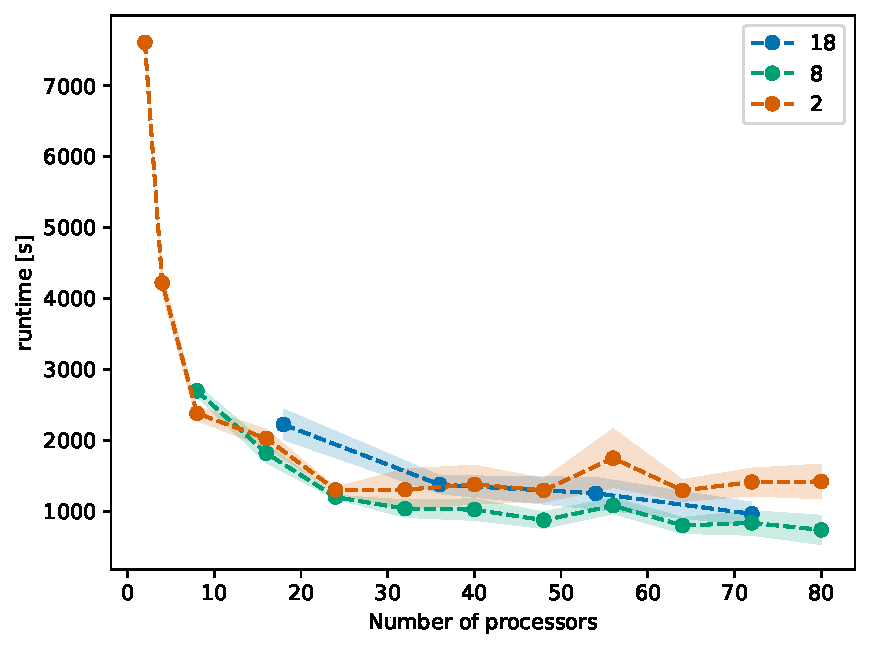
\includegraphics[width=\textwidth]{plots_ph/si_ph_bench_nk_absolute.pdf}
    %\end{subfigure}
    %\begin{subfigure}[b]{0.49\textwidth}
    %    \centering
    %    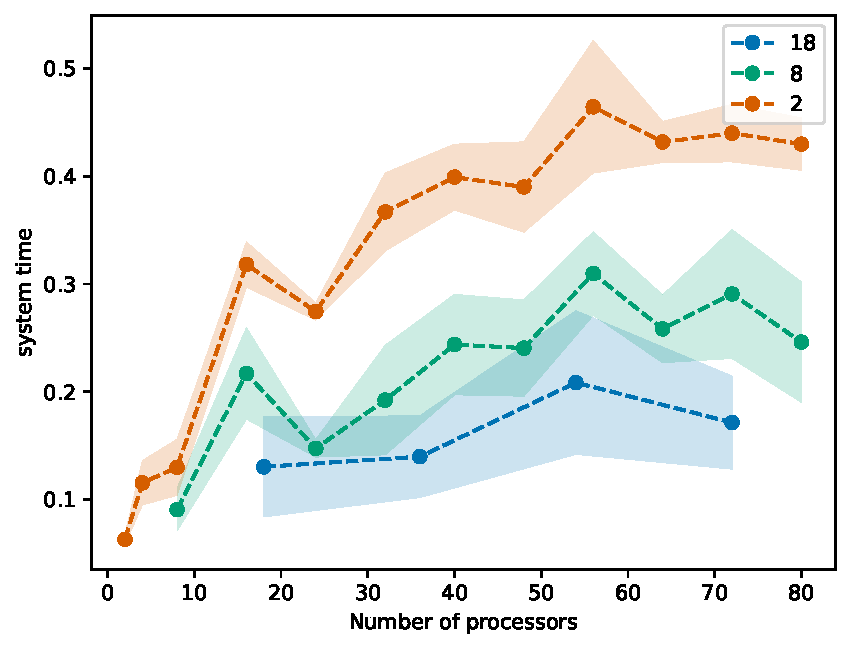
\includegraphics[width=\textwidth]{plots_ph/si_ph_bench_nk_wait.pdf}
    %\end{subfigure}
    \caption{Absolute runtime and wait time for the scalability test utilizing k-point parallelization for the Si benchmarking system with three sizes of processor pools, \emph{\QE compiled with \gls{oneapi} 2021.4, \texttt{nd 1}}}
    \label{fig:scaling_ph_nk_si_absolute_wait}
\end{figure}


The phonon benchmark has a similar runtime to the \texttt{PWscf} benchmark on \TaS shown in sec. \ref{sub:scf_scaling_k_point}, so comparison in wait time can reveal differences in the quality of parallelization between the two systems.
Whereas the \texttt{PWscf} benchmark on \TaS had wait time not exceeding about \(\SI{8}{\percent}\) of the \gls{wall_time}, the wait time shown in fig. \ref{fig:scaling_ph_nk_si_absolute_wait} between \(\SI{10}{\percent}\) and \(\SI{50}{\percent}\).
A possible explanation can be found how the time is actually spent during the calculation.
In the case of the phonon calculation on silicon, the time of one iteration is on the scale of seconds, whereas one iteration for the \texttt{PWscf} calculation on \TaS is about \(\SI{1}{\minute}\).
\todo{some more interpretation}

\subsection{Linear algebra parallelization}

\begin{figure}[htb!]
    \centering
    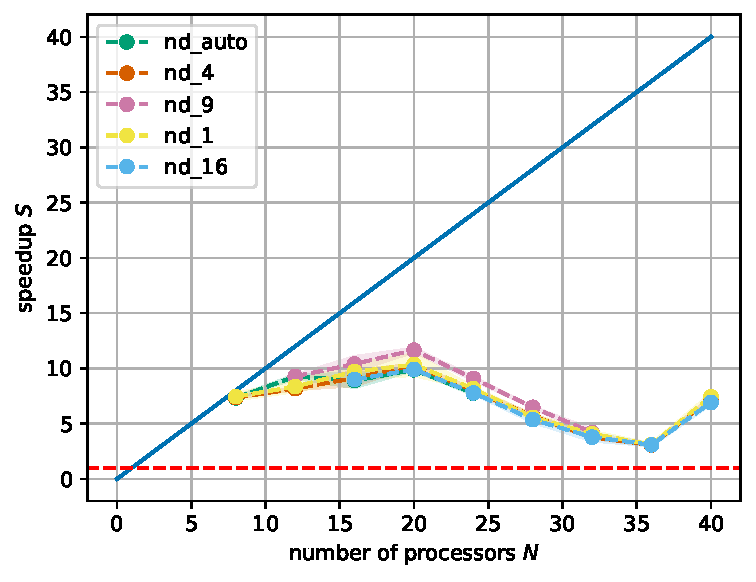
\includegraphics[width=0.75\textwidth]{plots_ph/si_ph_bench_nd_speedup.pdf}
    \caption{Scalability utilizing linear algebra parallelization for the Si benchmarking system, \emph{\QE compiled with \gls{oneapi} 2021.4, \texttt{nk 1}}}
    \label{fig:scaling_ph_nd_si}
\end{figure}
Fig. \ref{fig:scaling_ph_nd_si} shows that using linear algebra parallelization has so significant impact on the speedup, which is again in contrast to the results from sec. \ref{sec:scf_scaling_qe_parallelization}.
\todo{a bit more interpretation should be possible}

\subsection{Image parallelization}\label{sub:scaling_ph_images}

\todo{Better introduction}
When using image parallelization, \QE outputs a separate time report for every image, so one step is added to the analysis:
The total runtime of a calculation is determined by the longest running image, so speedup will be calculated using that value, but another important measure to evaluate is variation of times between images.
This is depicted in fig. \ref{fig:scaling_ph_ni_poolsize_8_si}.

\begin{figure}[ht!]
    \centering
    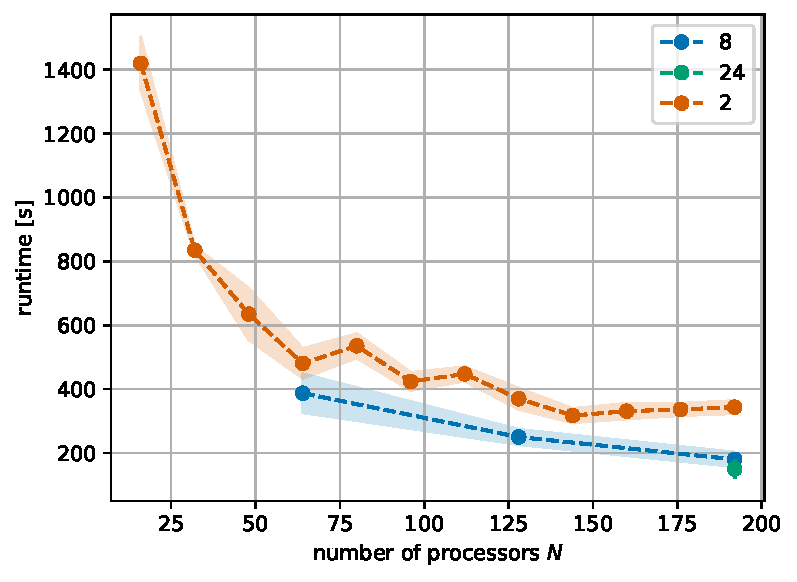
\includegraphics[width=0.8\textwidth]{plots_ph/si_ph_poolsize_8_images_distribution.pdf}
    \caption{Average runtime across images for the scalability test utilizing image and k point parallelization on the Si benchmarking system with three values of \emph{\texttt{ni}}, \emph{\QE compiled with \gls{oneapi} 2021.4, \texttt{nk, ni} chosen such that poolsize = 8, \texttt{nd 1}}}
    \label{fig:scaling_ph_ni_poolsize_8_si_distribution}
\end{figure}
As the times between images don't vary much, good load balancing between images can be assumed for the silicon benchmarking system.

With the maximum time across images, speedup is then calculated, shown in fig. \ref{fig:scaling_ph_ni_poolsize_8_si}.

\begin{figure}[ht!]
    \centering
    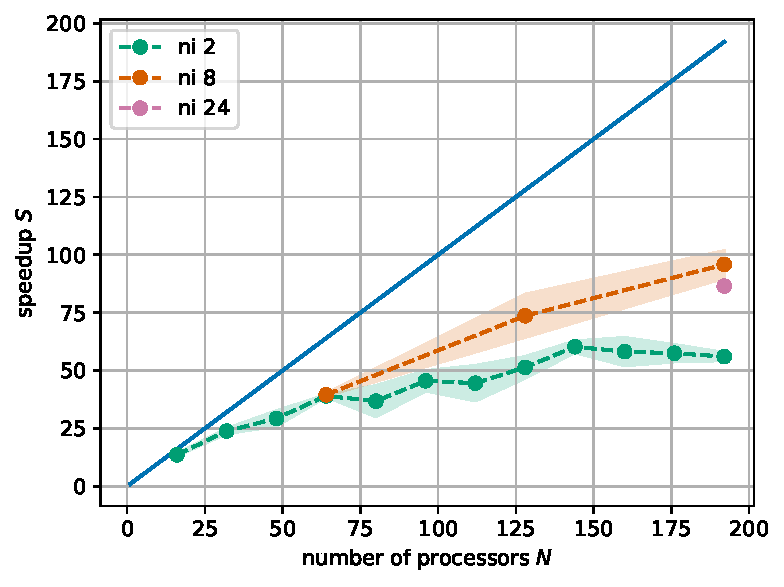
\includegraphics[width=0.8\textwidth]{plots_ph/si_ph_poolsize_8_bench_ni_speedup.pdf}
    \caption{Speedup calculated from the longest running image for the scalability test utilizing image and k point parallelization on the Si benchmarking system with three values of \emph{\texttt{ni}}, \emph{\QE compiled with \gls{oneapi} 2021.4, \texttt{nk, ni} chosen such that poolsize = 8, \texttt{nd 1}}}
    \label{fig:scaling_ph_ni_poolsize_8_si}
\end{figure}


\begin{figure}[ht!]
    \centering
    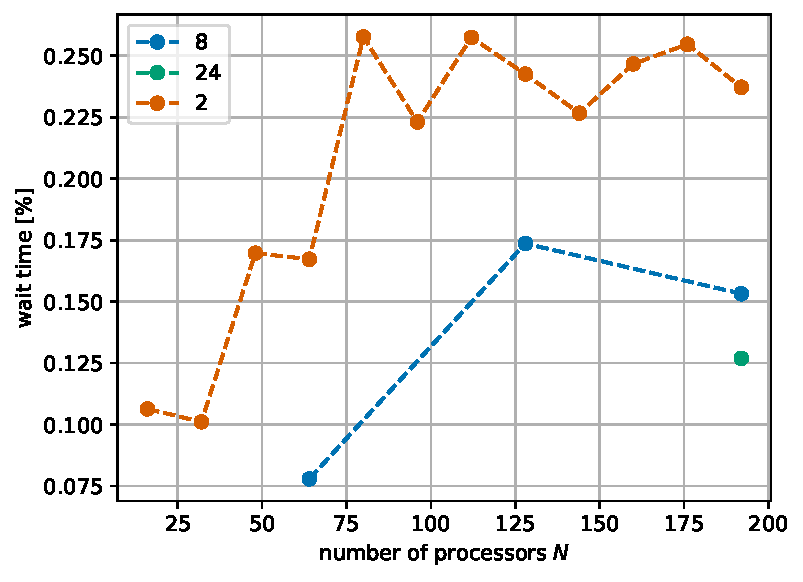
\includegraphics[width=0.8\textwidth]{plots_ph/si_ph_poolsize_8_bench_ni_wait.pdf}
    \caption{Wait time calculated from the longest running image for the scalability test utilizing image and k point parallelization on the Si benchmarking system with three values of \emph{\texttt{ni}}, \emph{\QE compiled with \gls{oneapi} 2021.4, \texttt{nk, ni} chosen such that poolsize = 8, \texttt{nd 1}}}
    \label{fig:scaling_ph_ni_poolsize_8_si_wait}
\end{figure}

\section{Phonon calculations on \TaS}

The results from the last section can be used to estimate good parallelization parameters for a phonon calculation at the \(\mathrm{\Gamma}\) point for \TaS in the charge density wave phase.
The calculations were run on 180 processors, once with the previous established optimal pool size of 36 and once with a pool size of 18 for comparison.
The relevant benchmark values for this calculation are listed in tab. \ref{tab:tas2_cdw_phonon_times}.

\begin{table}[ht!]
    \caption{CAPTION}
    \begin{tabular}{@{}lll@{}}
    \toprule
                 & runtime            & wait time \\ \midrule
    pool size 18 & \SI{3044}{\minute} & 0.16         \\
    pool size 36 & \SI{2020}{\minute} & 0.074
    \end{tabular}
    \label{tab:tas2_cdw_phonon_times}
\end{table}
In this calculation the need for a good choice of parallelization parameters becomes especially clear:
on the on the same number of processors, with the only difference in the choice of the parameter \texttt{nk}, the two calculations have a difference of \(\SI{17}{\hour}\).

\section{Conclusion: Parameters for optimal scaling}

\end{document}